\documentclass{article}

\usepackage{graphicx}
\usepackage{pdfpages}
\usepackage{amsmath}
\usepackage{amsfonts}
\usepackage{amssymb} 
\usepackage{centernot}
\usepackage{verbatim}
\usepackage{graphicx}
\usepackage[colorlinks]{hyperref}
\usepackage{caption}
\usepackage{subcaption}
\usepackage{titlesec}	
\usepackage{scrextend}
\usepackage{titlepic}
\usepackage{float}
\usepackage{wrapfig}
\usepackage{lscape}
\usepackage{rotating}
\usepackage{epstopdf}
\usepackage{pdflscape}
\usepackage[margin=1.0in]{geometry}


\title{\textbf{Catalyst Network - Technical White Paper}}
\date{\today}
\author{Joseph Kearney\thanks{joseph.kearney@atlascity.io} - Atlas City}


\begin{document}

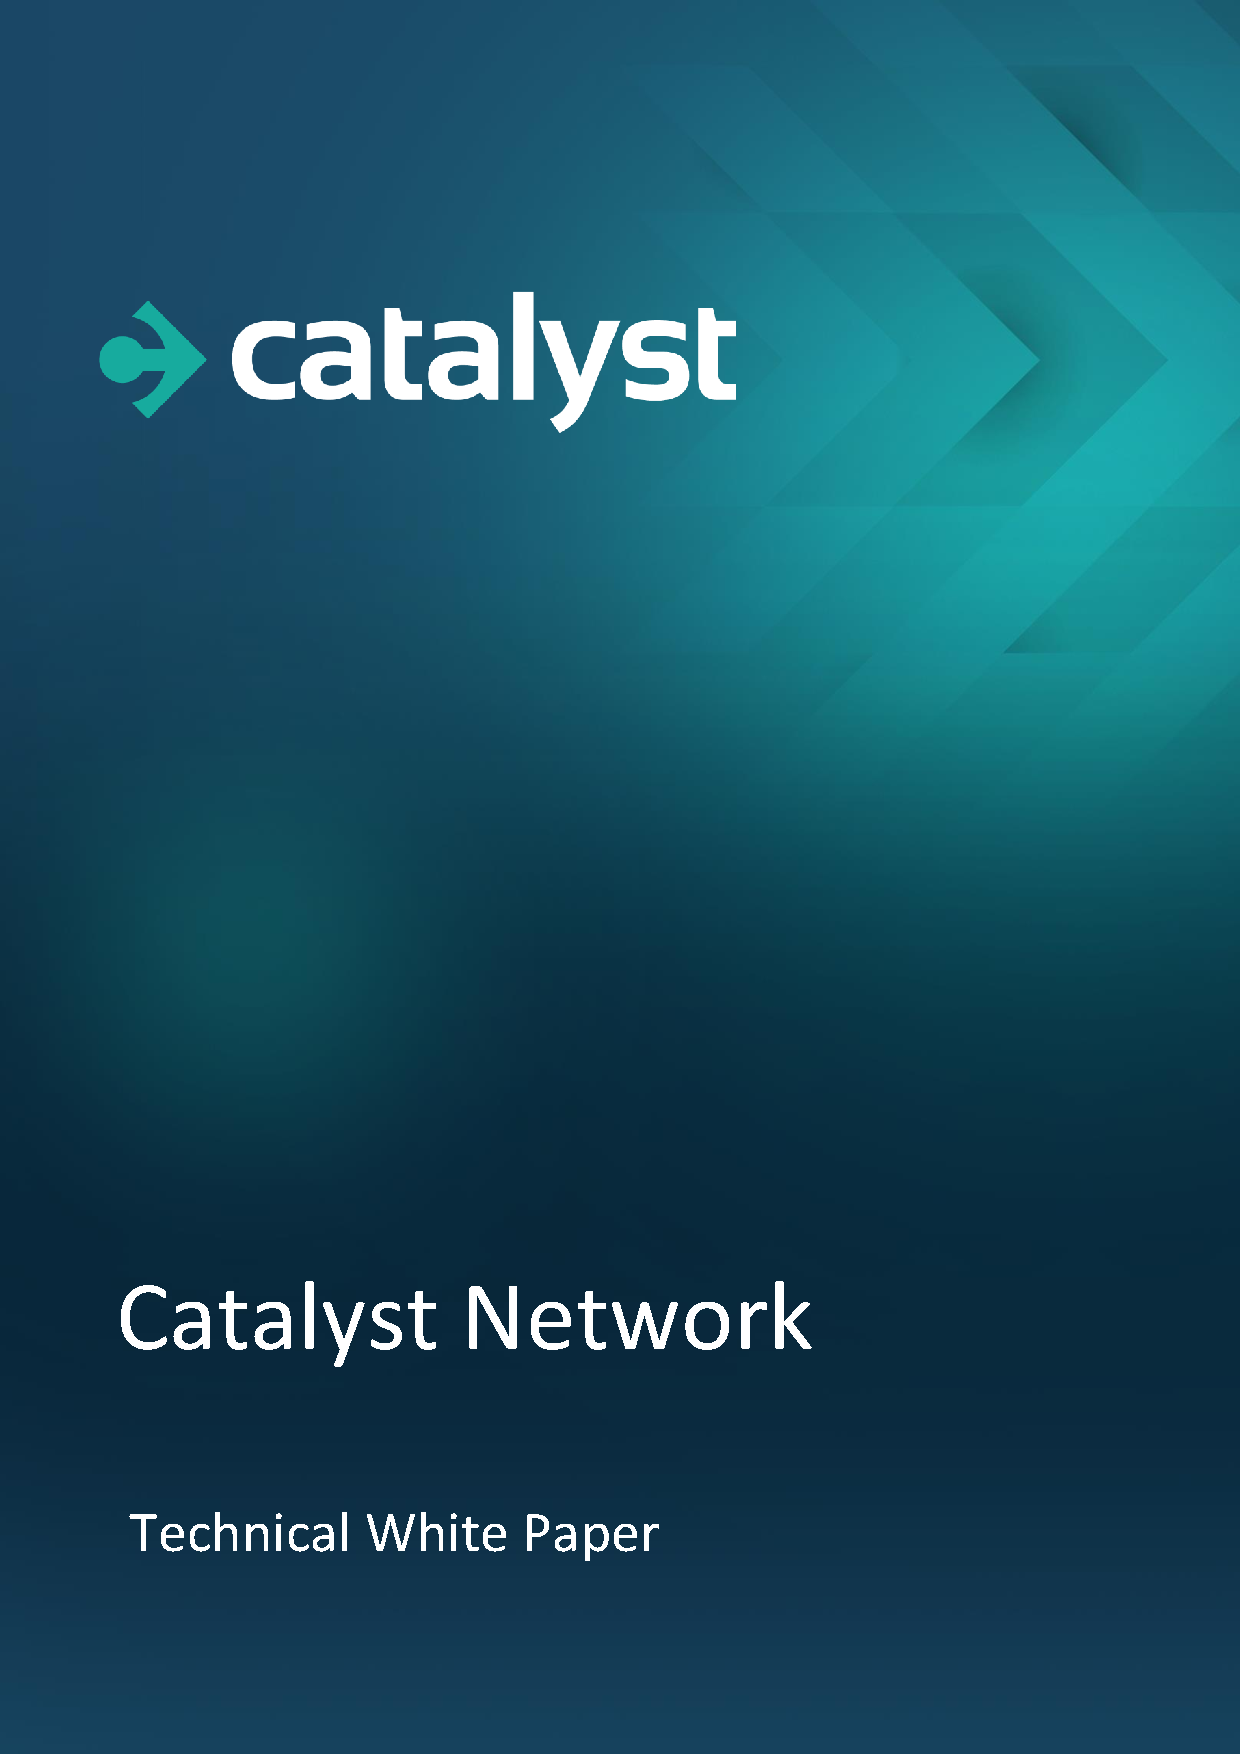
\includepdf [fitpaper=true] {cover-image}

\maketitle

\abstract 

hello

\newpage

\tableofcontents

\newpage

\section*{Introduction}

\section{Distributed File System}

Catalyst integrates its own DFS based on the InterPlanetery File System (IPFS) protocol \cite{benet2014ipfs}.

\section{KVM}

The Catalyst network 

\subsection{From the EVM}

\subsection{To the KVM}



\section{Catalyst Consensus Mechanism} 

On distributed networks there is no single point of trust to determine the validity of transactions, therefore concurrency must be ensured by other methods. Typically this requires a majority of the network's participants to agree on a particular update of the ledger and the account balances / holdings held within. Blockchain technologies generally employ Proof-of-Work (PoW) and occasionally Proof-of-Stake (PoS) mechanisms in order to gain consensus across a network. However, these methods are prone to increasing centralization at scale as well as in the case of PoW high energy consumption. Other networks employ a small amount of trusted nodes that ensure the validity of transactions, however this is highly centralised and almost as fallible as the single point of failure systems that DLT endeavors to avoid. \\

Catalyst integrates a newly designed consensus mechanism, based on Probabilistic Byzantine Fault Tolerance (PBFT).  This is a collaborative rather than competitive protocol, meaning that all honest work performed by nodes on the network benefits the security of the network and that all participating nodes are rewarded equally. For each ledger cycle a random selection of worker nodes are selected, the nodes become the producers for a cycle or number of cycles. The producer nodes perform work in the form of compiling and validating transaction thereby extracting a ledger state change for that cycle. \\

The protocol is split into four distinct phases:

\begin{itemize}

\item Construction Phase - Producer nodes that have been selected create what they believe to be the correct update of the ledger. They then distribute this proposed ledger update in the form of it hash digest.
\item Campaigning Phase - Producer nodes designate and declare what they believe to be the most popular ledger state update. 
\item Voting Phase - 	
\item Synchronisation Phase - In this phase the producers who have computed the correct ledger update can broadcast this update the rest of the network. 

\end{itemize} 

\subsection{Notation} 

\subsection{Producer Node Selection} 

%%%%%%%%%%%%%%%%%%%%%%%%%%%%%%%%%%%%%%%%%%%%%%%%%%%%%%%%%%%%%%%%%%%%%%%%%%%%%%%%%%

\subsection{Construction Phase}

The first phase of the Catalyst consensus algorithm is the Construction Phase. Within which the selected producer nodes  $P_j~\forall j \in P$ calculate their proposed ledger state update or their local ledger state update. This is done by aggregating and validating all transactions that have occurred during a set time period. These transactions assuming their validity are integrated into the producers local ledger state update. From which they can create a hash of the update. This hash digest represents what they believe to be the correct update and is broadcast to the other producer nodes during for that cycle. Assuming the collision free nature of hash functions, the only mechanism for multiple producer nodes to have the same local ledger state update is by both using the same set of transactions. \\

The first phase starts at $t = t_p = t_{n,0}$ and lasts for a period of time $\Delta t_{p}$, therefore ending at $t_p+\Delta t_{p}$.

\subsubsection{Local partial ledger state update generation and broadcast}

Each producer in the set of producers $P$ follows the same protocol. The construction phase begins with producer $P_i$ beginning their construction phase by flushing their mempool. This mempool is made up of $\{T_i\}_{i=1,..,n}$ [BE MORE CLEAR WITH THIS DEF] where $n$ is the number of transactions that have been broadcast to the network and have been stored by $P_i$. These transaction are used to create $P_i$'s local ledger state update $U_i$.  \\

The producer at this point also creates a hash trees $d_i$, this is to store the the signatures that are extracted from each transaction in $T_i$. A salt $\sigma$ is created utilizing a pseudo-random number generator using the previous ledger state update $U_{n-1}$ as its seed. $P_i$ then follows the following steps: 

\begin{enumerate}
\item Producer $P_i$ verifies that each transaction in $\{T_i\}_{i=1,..,n}$ is valid following the rules set out in [ADD CITATION FOR GITHUB WITH VALID TRANSACTION RULES]. From each of the transactions in $\{T_i\}_{i=1,..,n}$ the entries that constitute the transaction are extracted to form a list $\{E_\alpha\}_{\alpha=1,...,m}$. The producer should therefore end up with as many lists as there are valid transactions from $\{T_i\}_{i=1,..,n}$. each signature from the transactions are also extracted and added to $d_i$.

\item $P_i$ for each $\{E_\alpha\}$ it created then creates a corresponding hash digest as: 
\begin{center}
$O_\alpha [CHANGE THIS VARIABLE] = \mathcal{H}[E_\alpha~||~\sigma]$
\end{center}

Each pair ($E_\alpha,O_\alpha$) is added to a list $L_i$. 

\item $P_i$ then sorts list $L_i$ into lexicographical order according the hash values $O_\alpha$.

\item The producer $P_i$ then extracts the transaction fee value from each transaction in $\{Tx_i\}$ to create $v_i$ which is the total sum of all transaction fees. 

\item The local ledger state update $U_i$ for producer $P_i$ can then be calculated. Firstly the list $L_i$ is concatenated with the hashtree $d_i$ and a hash digest is created as: 

\begin{center}
$U_i = \mathcal{H}(L_i~||~d_i)$
\end{center}  

$U_i$ is then concatenated with $P_i$'s unique peer identifier $Id_i$ to create:

\begin{center} 
$h_i = U_i ~||~Id_i$
\end{center}

\item $h_i$ is then broadcast to the other producer nodes on the network. 
\end{enumerate}

\subsubsection{Partial ledger state update collection}

[THIS SECTION NEEDS IMPROVING]

Producer $P_i$ also collects other producers partial ledger update values. At most they will collect $P-1$ values. Optimally every producer in $P$ will receive the same set of transactions therefore for every $P_i \in P_{1,..,j}$ will have the same partial ledger update $U_j$. However this is unlikely due to all transaction not being received by a small group of nodes. Equally they may not hold $G_i$ where  $\{G_i\}_{i=h_1,..,h_j}$, meaning they may not receive a proposed update from all candidates. 

%%%%%%%%%%%%%%%%%%%%%%%%%%%%%%%%%%%%%%%%%%%%%%%%%%%%%%%%%%%%%%%%%%%%%%%%%%%%%%%%%%%

\subsection{Campaigning Phase}

The second phase of the consensus mechanism is where producer $P_i$ designates a candidate for what it calculates to be the most popular ledger state update. \\

\subsubsection{Local candidate generation and broadcast}

Beginning this phase producer $P_i$ has a set of partial ledger updates $G_i$ that it has received from other producer nodes. Each $h_j$ within $G_i$ contains a producers hash of the proposed update ($U_j$ and their peer identifier ($Id_j$). The most popular $U_j$ value can be found, this gives us $U_j^{maj}$ from there the subset $G_{maj}$ can be created, which is the amount of votes for the most popular update. Two thresholds must be considered first is $G_min$ this is the minimum amount of updates it has received from other producers in order to generate a valid candidate. The second is $G_{thresh}$ this is the threshold value for which a minimum number of votes must be in favor of $G_{maj}$ which the most popular vote found within $G_i$.  So in order to proceed with declaring a candidate $G_i > G_{min}$ and $G_{maj} > G_{thresh}$. \\

If the thresholds are met the following can take place:

\begin{enumerate}
\item $P_i$ creates a list $\mathcal{L}_i(prod)$. To this list $P_i$ appends the identifier of any producer that correctly sent the $U_j$ value that equals $U_j^{maj}$. If $P_i$'s $U_i$ value is also the same as $U_j^{maj}$ then they should append their own $Id_i$.
\item Producer $P_i$ then creates their candidate for the ledger update $c_i$ which is calculated as $c_i = U_j^{maj}~||~\#(\mathcal{L}_i(prod))~||~Id_i$
\item Producer $P_i$ will then broadcast their preferred update $c_i$ to the other producers. 
\end{enumerate}



\subsubsection{Candidate collection}

$P_i$ during this phase will be collecting the $c_j$ values from other producers. At the end of this cycle $P_i$ will hold a set $V_i$ candidates.


%%%%%%%%%%%%%%%%%%%%%%%%%%%%%%%%%%%%%%%%%%%%%%%%%%%%%%%%%%%%%%%%%%%%%%%%%%%%%

\subsection{Voting Phase}

The third phase of the ledger cycle is the Voting Phase within which a producer $P_i$ from the $V_i$ candidates it has recieved decides on what it belives should be the global ledger state update i.e. the update that should be applied to the ledger for that cycle. 



\subsection{Synchronisation Phase}

\bibliography{catalyst-technical-whitepaper}
\bibliographystyle{ieeetr}

\end{document}